\documentclass[12pt]{article}
\usepackage[utf8]{inputenc}
\usepackage{float}
\usepackage{amsmath}
\usepackage[shortlabels]{enumitem}
\usepackage[dvips]{graphicx}
\usepackage{fancybox}
\usepackage{verbatim}
\usepackage{array}
\usepackage{latexsym}
\usepackage{alltt}
\usepackage{hyperref}
\usepackage{textcomp}
\usepackage{color}
\usepackage{amsfonts}
\usepackage{tikz}
\usepackage{blkarray}
%\usepackage{a4wide}
\usepackage{epsfig}
%\usepackage{dsfont}
\usepackage{caption}
\usepackage{subcaption}
%\usepackage{fullpage}
\usepackage{hyperref}
\usepackage{textcomp}
\usepackage{listings}



\usepackage[hmargin=3cm,vmargin=6.0cm]{geometry}
%\topmargin=0cm
\topmargin=-2cm
\addtolength{\textheight}{6.5cm}
\addtolength{\textwidth}{2.0cm}
%\setlength{\leftmargin}{-5cm}
\setlength{\oddsidemargin}{0.0cm}
\setlength{\evensidemargin}{0.0cm}

%misc libraries goes here




\begin{document}

\section*{Student Information } 
%Write your full name and id number between the colon and newline
%Put one empty space character after colon and before newline
Full Name :  Berk Ulutaş \\
Id Number :  2522084 \\

% Write your answers below the section tags
\section*{Answer 1}
\begin{enumerate} [a)]
    \item Sum of degrees of all nodes = 14
    \begin{itemize}
        \item deg(a) = 3
        \item deg(b) = 3
        \item deg(c) = 3
        \item deg(d) = 2
        \item deg(e) = 3
    \end{itemize}
    \item The number of non-zero entries in the adjacency matrix is 14.
    

    \[
    \begin{blockarray}{cccccc}
     & a & b & c & d & e \\
    \begin{block}{c[ccccc]}
      a & 0 & 1 & 1 & 0 & 1  \\
      b & 1 & 0 & 1 & 0 & 1 \\
      c & 1 & 1 & 0 & 1 & 0 \\
      d & 0 & 0 & 1 & 0 & 1 \\
      e & 1 & 1 & 0 & 1 & 0 \\
    \end{block}
    \end{blockarray}
     \]

    \item The number of non-zero entries in the incidence matrix is 21.
    \begin{figure}[H]
    	\centering
    	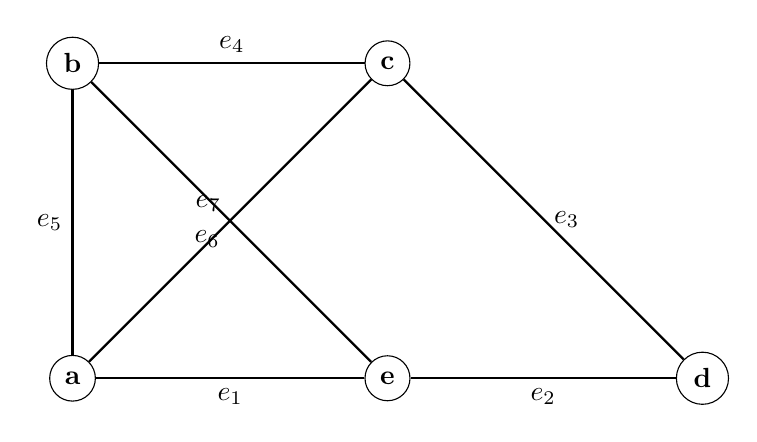
\begin{tikzpicture}
    	
    	\node[shape=circle,draw=black] (b) at (0, 4)     {\textbf{b}};
    	\node[shape=circle,draw=black] (c) at (4, 4)     {\textbf{c}};
    	\node[shape=circle,draw=black] (d) at (8, 0)     {\textbf{d}};
    	\node[shape=circle,draw=black] (e) at (4, 0)     {\textbf{e}};
    	\node[shape=circle,draw=black] (a) at (0, 0)     {\textbf{a}};
    	
    	\path[-, thick] (a) edge node[below]{$e_1$} (e);
    	\path[-, thick] (e) edge node[below]{$e_2$}(d);
    	\path[-, thick] (c) edge node[right]{$e_3$}(d);
    	\path[-, thick] (b) edge node[above]{$e_4$}(c);
    	\path[-, thick] (a) edge node[left]{$e_5$}(b);
    	\path[-, thick] (a) edge node[below left]{$e_6$}(c);
    	\path[-, thick] (b) edge node[above left]{$e_7$}(e);
    	
    	\end{tikzpicture} 
    	\caption{Graph G in Q1.}	
    	\label{fig:g1.1}
    \end{figure}

    \[
    \begin{blockarray}{cccccccc}
     & e_1 & e_2 & e_3 & e_4 & e_5 & e_6 & e_7 \\
    \begin{block}{c[ccccccc]}
      a & 1 & 0 & 0 & 0 & 1 & 1 & 0 \\
      b & 0 & 0 & 0 & 1 & 1 & 0 & 1 \\
      c & 0 & 0 & 1 & 1 & 0 & 1 & 0 \\
      d & 0 & 1 & 1 & 0 & 0 & 0 & 0 \\
      e & 1 & 1 & 0 & 0 & 0 & 0 & 1 \\
    \end{block}
    \end{blockarray}
     \]

     \item No!
     \begin{itemize}
         \item A complete graph with 4 vertices has $C(4,2) =6$ edges. And a complete graph with 5 vertices has $C(5,2) =10$ edges.
         \item Initially $G$ has 5 vertices and 7 edges. 4 of the vertices has degree 3 and other vertex has degree 2.
         \item $G$'s itself is not a complete graph since it does not have enough edges.
         \item We can obtain subgraphs of $G$ removing a vertex.
         \item If we remove one of the degree 3 vertex. The remaining subgraph has 4 vertices and 4 edges. It cannot be complete graph since it doesn't have 6 edges.
         \item If we remove degree 2 vertex. The remaining subgraph has 4 vertices and 5 edges. Similarly it cannot be complete graph since it doesn't have 6 edges.
         \item So we can conclude that the graph $G$ does not have a subgraph with at least four vertices.
     \end{itemize}
     \item $G$ is not bipartite since it does not satisfy graph color test
     \begin{itemize}
         \item Pick vertex b color it red and color adjacent vertices blue.
         \item Since a and c are adjacent vertices and same color. There is no need to continue. The graph $G$ is not bipartite.
     \end{itemize}
     \begin{figure}[H]
	\centering
	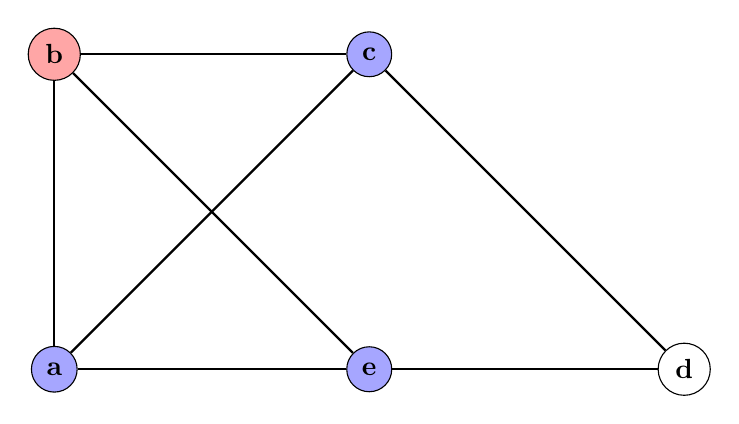
\begin{tikzpicture}
	
	\node[shape=circle,draw=black, fill=red!35] (b) at (0, 4)     {\textbf{b}};
	\node[shape=circle,draw=black, fill=blue!35] (c) at (4, 4)     {\textbf{c}};
	\node[shape=circle,draw=black] (d) at (8, 0)     {\textbf{d}};
	\node[shape=circle,draw=black, fill=blue!35] (e) at (4, 0)     {\textbf{e}};
	\node[shape=circle,draw=black, fill=blue!35] (a) at (0, 0)     {\textbf{a}};
	
	\path[-, thick] (a) edge (e);
	\path[-, thick] (e) edge (d);
	\path[-, thick] (c) edge (d);
	\path[-, thick] (b) edge (c);
	\path[-, thick] (a) edge (b);
	\path[-, thick] (a) edge (c);
	\path[-, thick] (b) edge (e);
	
	\end{tikzpicture} 
	\caption{Graph G in Q1.}	
	\label{fig:g1.0}
\end{figure}
     \item For each edge in the undirected graph G, there are two possible directions that the edge can be oriented in a directed graph. Thus, for the graph G with 7 edges, there are $2^7 = 128$ possible directed graphs that have G as their underlying undirected graph.
     \item The length of the simple longest path in G is 6. One of the possible path is $(a,b,e,a,c,d,e)$
     \item Number of connected components of G is 1.
     \begin{figure}[H]
    	\centering
    	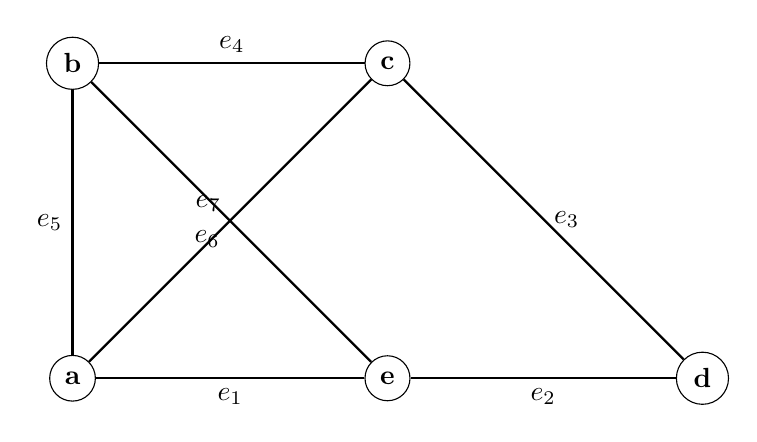
\begin{tikzpicture}
    	
    	\node[shape=circle,draw=black] (b) at (0, 4)     {\textbf{b}};
    	\node[shape=circle,draw=black] (c) at (4, 4)     {\textbf{c}};
    	\node[shape=circle,draw=black] (d) at (8, 0)     {\textbf{d}};
    	\node[shape=circle,draw=black] (e) at (4, 0)     {\textbf{e}};
    	\node[shape=circle,draw=black] (a) at (0, 0)     {\textbf{a}};
    	
    	\path[-, thick] (a) edge node[below]{$e_1$} (e);
    	\path[-, thick] (e) edge node[below]{$e_2$}(d);
    	\path[-, thick] (c) edge node[right]{$e_3$}(d);
    	\path[-, thick] (b) edge node[above]{$e_4$}(c);
    	\path[-, thick] (a) edge node[left]{$e_5$}(b);
    	\path[-, thick] (a) edge node[below left]{$e_6$}(c);
    	\path[-, thick] (b) edge node[above left]{$e_7$}(e);
    	
    	\end{tikzpicture} 
    	\caption{Graph G in Q1.}	
    	\label{fig:g1}
    \end{figure}
     \begin{itemize}
         \item Let each vertex in G be a disjoint set. $\{ a\},\{ b\},\{ c\},\{ d\},\{ e\}$. For each edge (u, v), if the vertices u and v are in different sets, merge the sets containing u and v.
         \begin{itemize}
             \item for $e_1$: merge $\{ a\}$ and $\{ e\}$. $$\{ a,e\},\{ b\},\{ c\},\{ d\}$$
             \item for $e_2$: merge $\{ a,e\}$ and $\{ d\}$. $$\{ a,d,e\},\{ b\},\{ c\}$$
             \item for $e_3$: merge $\{ a,d,e\}$ and $\{ c\}$. $$\{ a,c,d,e\},\{ b\}$$
             \item for $e_4$: merge $\{ a,c,d,e\}$ and $\{ b\}$. $$\{ a,b,c,d,e\}$$
             \item since there is only one set no need to continue.
         \end{itemize}
         \item Thus, there is one connected component which is $\{ a,b,c,d,e\}$
     \end{itemize}
     \item No there is not an Euler circuit in $G$.
     \begin{itemize}
         \item Theorem 1 from the section 10.5 of the textbook states that "A connected multigraph with at least two vertices has an Euler circuit if and only if each of its vertices has even degree."
         \item From theorem 1 we can conclude that $G$ has not an Euler circuit since it has vertices which has odd degree. Such as $(a,b,c,e)$
     \end{itemize}
     \item No there is not an Euler path in $G$.
     \begin{itemize}
        \item Theorem 2 from the section 10.5 of the textbook says "A connected multigraph has an Euler path but not an Euler circuit if and only if it has exactly
two vertices of odd degree."
        \item Since vertices $a,b,c,e$ has odd degree and there are more than two vertices of odd degree we can conclude that the graph $G$ has not an Euler path.
     \end{itemize}
     \item Yes. $(d,c,b,a,e,d)$ is a Hamilton circuit.
     \item Yes. $(d,c,b,a,e)$ is a Hamilton path.
     
\end{enumerate}


\section*{Answer 2}

Let $G = (V_1, E_1)$ and $H = (V_2, E_2)$. Since $G$ and $H$ are simple graphs, if we can find a \emph{one-to-one} and \emph{onto} function $f$ from $V_1$ to $V_2$ with property that $a$ and $b$ are adjacent in $G_1$ if and only if $f(a)$ and $f(b)$ are adjacent in $G_2$, for all $a$ and $b$ in $V_1$ we can show that $G$ and $H$ are isomorphic. The graph $G$ has 5 vertices with degree 2 and 5 edges. Similarly the graph $H$ has 5 vertices with degree 2 and 5 edges. \\


Let $f$ be \emph{one-to-one} and \emph{onto} function from $V_1$ to $V_2$. Let the correspondence between graphs:
\begin{itemize}
    \item $f(a) = a'$
    \item $f(b) = b'$
    \item $f(c) = c'$
    \item $f(d) = d'$
    \item $f(e) = e'$
\end{itemize}

This correspondence preserves adjacency since:
\begin{itemize}
    \item $a$ is adjacent to $b$ and $e$ in G and $f(a) = a'$ is adjacent to $f(b) = b'$ and $f(e) = e'$ in H.
    \item $b$ is adjacent to $a$ and $c$ in G and $f(b) = b'$ is adjacent to $f(a) = a'$ and $f(c) = c'$ in H.
    \item $c$ is adjacent to $d$ and $b$ in G and $f(c) = c'$ is adjacent to $f(d) = d'$ and $f(b) = b'$ in H.
    \item $d$ is adjacent to $c$ and $e$ in G and $f(d) =d'$ is adjacent to $f(c) = c'$ and $f(e) = e'$ in H.
    \item $e$ is adjacent to $a$ and $d$ in G and $f(e) = e'$ is adjacent to $f(a) = a'$ and $f(d) = d'$ in H.
\end{itemize}
Hence $G$ and $H$ are isomorphic.
\begin{figure}[H]
	\centering
	\begin{subfigure}[b]{0.4\textwidth}
         \centering
         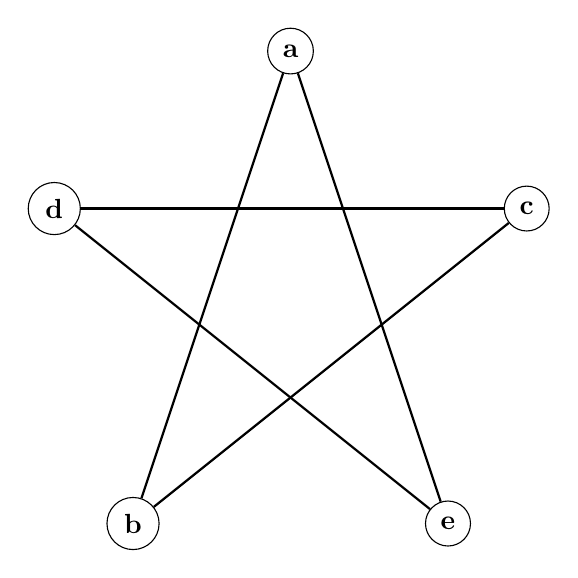
\begin{tikzpicture}
	
	\node[shape=circle,draw=black] (b) at (2, 0)     {\textbf{b}};
	\node[shape=circle,draw=black] (e) at (6, 0)     {\textbf{e}};
	\node[shape=circle,draw=black] (d) at (1, 4)     {\textbf{d}};
	\node[shape=circle,draw=black] (c) at (7, 4)     {\textbf{c}};
	\node[shape=circle,draw=black] (a) at (4, 6)     {\textbf{a}};
	
	\path[-, thick] (a) edge (b);
	\path[-, thick] (b) edge (c);
	\path[-, thick] (c) edge (d);
	\path[-, thick] (d) edge (e);
	\path[-, thick] (e) edge (a);
	
	\end{tikzpicture} 
         \caption{G}
         \label{fig:g}
     \end{subfigure}
     \hfill
     \begin{subfigure}[b]{0.4\textwidth}
         \centering
         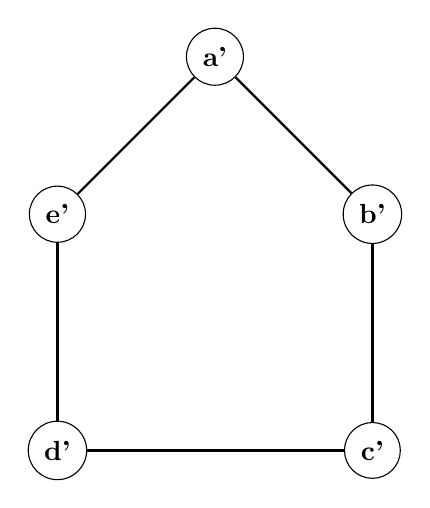
\begin{tikzpicture}
	
	\node[shape=circle,draw=black] (d') at (2, 0)     {\textbf{d'}};
	\node[shape=circle,draw=black] (c') at (6, 0)     {\textbf{c'}};
	\node[shape=circle,draw=black] (e') at (2, 3)     {\textbf{e'}};
	\node[shape=circle,draw=black] (b') at (6, 3)     {\textbf{b'}};
	\node[shape=circle,draw=black] (a') at (4, 5)     {\textbf{a'}};
	
    \path[-, thick] (a') edge (b');
    \path[-, thick] (a') edge (e');
    \path[-, thick] (b') edge (c');
    \path[-, thick] (d') edge (e');
    \path[-, thick] (c') edge (d');
	
	\end{tikzpicture} 
         \caption{H}
         \label{fig:h}
     \end{subfigure}
     \caption{Graph $G$ and $H$.}
        \label{fig:g2}
\end{figure}
\setcounter{figure}{0}
\section*{Answer 3}
\begin{enumerate} [1)]
    \item Set the distance of the neighbors of $s$ to the length of the edge between $s$ and them. Mark $s$ visited since shortest path to $s$ is found which is 0. For other vertices set the distance $\infty$
    \begin{center}
        \begin{tabular}{|c|c|c|c|}
        \hline
        \textbf{Vertex} & \textbf{Distance} & \textbf{Prev.} & \textbf{Visited}\\ \hline
        $\rightarrow$ s & 0 & - & \textbf{T}\\ \hline
        \textbf{*u} & \textbf{4} & \textbf{(s)} & F\\ \hline
        \textbf{*v} & \textbf{5} & \textbf{(s)} & F\\ \hline
        \textbf{*w} & \textbf{3} & \textbf{(s)} & F\\ \hline
        x & $\infty$ & - & F \\ \hline
        y & $\infty$ & - & F\\ \hline
        z & $\infty$ & - & F\\ \hline
        t & $\infty$ & - & F\\ \hline
        \end{tabular}
    \end{center}
    \item The next vertex is $w$ since it has minimum distance in unvisited vertices. Update distances and previous vertex for vertices $x$ and $z$ since new distances are smaller than previous distances. Mark $w$ visited since shortest path to $w$ is found which is 3.
    \begin{center}
        \begin{tabular}{|c|c|c|c|}
        \hline
        \textbf{Vertex} & \textbf{Distance} & \textbf{Prev.} & \textbf{Visited}\\ \hline 
        s & 0 & - & T\\ \hline
        u & 4 & (s) & F\\ \hline
        v & 5 & (s) & F\\ \hline
        $\rightarrow$w & 3 & (s) & \textbf{T}\\ \hline
        \textbf{*x} & \textbf{11} & \textbf{(w)} & F \\ \hline
        y & $\infty$ & - & F\\ \hline
        \textbf{*z} & \textbf{15} & \textbf{(w)} & F\\ \hline
        t & $\infty$ & - & F\\ \hline
        \end{tabular}
    \end{center}
    \item The next vertex is $u$ since it has minimum distance in unvisited vertices. Update distance and previous vertex for vertex $y$ since new distance is smaller than previous distance. Mark $u$ visited since shortest path to $u$ is found which is 4.
    \begin{center}
        \begin{tabular}{|c|c|c|c|}
        \hline
        \textbf{Vertex} & \textbf{Distance} & \textbf{Prev.} & \textbf{Visited}\\ \hline
        s & 0 & - & T\\ \hline
        $\rightarrow$u & 4 & (s) & \textbf{T}\\ \hline
        v & 5 & (s) & F\\ \hline
        w & 3 & (s) & T\\ \hline
        x & 11 & (w) & F \\ \hline
        \textbf{*y} & \textbf{15} & \textbf{(u)} & F\\ \hline
        z & 15 & (w) & F\\ \hline
        t & $\infty$ & - & F\\ \hline
        \end{tabular}
    \end{center}
    \item The next vertex is $v$ since it has minimum distance in unvisited vertices. Update distances and previous vertex for vertices $x$ and $y$ since new distances is smaller than previous distances. Mark $v$ visited since shortest path to $v$ is found which is 5.
    \begin{center}
        \begin{tabular}{|c|c|c|c|}
        \hline
        \textbf{Vertex} & \textbf{Distance} & \textbf{Prev.} & \textbf{Visited}\\ \hline
        s & 0 & - & T\\ \hline
        u & 4 & (s) & T\\ \hline
        $\rightarrow$v & 5 & (s) & \textbf{T}\\ \hline
        w & 3 & (s) & T\\ \hline
        \textbf{*x} & \textbf{7} & \textbf{(v)} & F \\ \hline
        \textbf{*y} & \textbf{11} & \textbf{(v)} & F\\ \hline
        z & 15 & (w) & F\\ \hline
        t & $\infty$ & - & F\\ \hline
        \end{tabular}
    \end{center}
    \item The next vertex is $x$ since it has minimum distance in unvisited vertices. Update distances and previous vertex for vertices $y$ and $z$ since new distance is smaller than previous distances. Mark $x$ visited since shortest path to $x$ is found which is 7.
    \begin{center}
        \begin{tabular}{|c|c|c|c|}
        \hline
        \textbf{Vertex} & \textbf{Distance} & \textbf{Prev.} & \textbf{Visited}\\ \hline
        s & 0 & - & T\\ \hline
        u & 4 & (s) & T\\ \hline
        v & 5 & (s) & T\\ \hline
        w & 3 & (s) & T\\ \hline
        $\rightarrow$x & 7 & (v) & \textbf{T} \\ \hline
        \textbf{*y} & \textbf{8} & \textbf{(x)} & F\\ \hline
        \textbf{*z} & \textbf{13} & \textbf{(x)} & F\\ \hline
        t & $\infty$ & - & F\\ \hline
        \end{tabular}
    \end{center}
    \item The next vertex is $y$ since it has minimum distance in unvisited vertices. Update distances and previous vertex for vertices $z$ and $t$ since new distance is smaller than previous distances. Mark $y$ visited since shortest path to $y$ is found which is 8.
    \begin{center}
        \begin{tabular}{|c|c|c|c|}
        \hline
        \textbf{Vertex} & \textbf{Distance} & \textbf{Prev.} & \textbf{Visited}\\ \hline
        s & 0 & - & T\\ \hline
        u & 4 & (s) & T\\ \hline
        v & 5 & (s) & T\\ \hline
        w & 3 & (s) & T\\ \hline
        x & 7 & (v) & T \\ \hline
        $\rightarrow$y & 8 & (x) & \textbf{T}\\ \hline
        \textbf{*z} & \textbf{12} & \textbf{(y)} & F\\ \hline
        \textbf{*t} & \textbf{17} & \textbf{(y)} & F\\ \hline
        \end{tabular}
    \end{center}
    \item The next vertex is $z$ since it has minimum distance in unvisited vertices. Update distances and previous vertex for vertex $t$ since new distance is smaller than previous distance. Mark $z$ visited since shortest path to $z$ is found which is 12.
    \begin{center}
        \begin{tabular}{|c|c|c|c|}
        \hline
        \textbf{Vertex} & \textbf{Distance} & \textbf{Prev.} & \textbf{Visited}\\ \hline
        s & 0 & - & T\\ \hline
        u & 4 & (s) & T\\ \hline
        v & 5 & (s) & T\\ \hline
        w & 3 & (s) & T\\ \hline
        x & 7 & (v) & T \\ \hline
        y & 8 & (x) & T\\ \hline
        $\rightarrow$z & 12 & (y) & \textbf{T}\\ \hline
        \textbf{*t} & \textbf{15} & \textbf{(z)} & F\\ \hline
        \end{tabular}
    \end{center}
    \item The next vertex is $t$ and there are no unvisited neighbor vertex. Mark $t$ visited. So the algorithm finished.
    \begin{center}
        \begin{tabular}{|c|c|c|c|}
        \hline
        \textbf{Vertex} & \textbf{Distance} & \textbf{Prev.} & \textbf{Visited}\\ \hline
        s & 0 & - & T\\ \hline
        u & 4 & (s) & T\\ \hline
        v & 5 & (s) & T\\ \hline
        w & 3 & (s) & T\\ \hline
        x & 7 & (v) & T \\ \hline
        y & 8 & (x) & T\\ \hline
        z & 12 & (y) & T\\ \hline
        t & 15 & (z) & T\\ \hline
        \end{tabular}
    \end{center}
\end{enumerate}
To find shortest path vertex $s$ to vertex $t$. We need to follow the previous vertices until we find $s$ from $t$ and reverse. 
The shortest path vertex $s$ to vertex $t$ is $(s,v,x,y,z,t)$ with distance 15.


\section*{Answer 4}
\subsection*{a)} Choosed Prim's Algorithm.
\begin{center}
        \begin{tabular}{|c|c|c|}
        \hline
        \textbf{Order} & \textbf{Edge} & \textbf{Weight}\\ \hline
        1 & (b,c) & 2 \\ \hline
        2 & (c,f) & 2 \\ \hline
        3 & (c,d) & 3 \\ \hline
        4 & (d,k) & 2 \\ \hline
        5 & (a,b) & 3 \\ \hline
        6 & (f,g) & 4 \\ \hline
        7 & (f,j) & 3 \\ \hline
        8 & (f,e) & 4 \\ \hline
        9 & (f,i) & 4 \\ \hline
        10 & (i,h) & 2 \\ \hline
        \end{tabular}
    \end{center}
\subsection*{b)} Minimum Spanning Tree with total weight 29.
\begin{figure}[H]
	\centering
	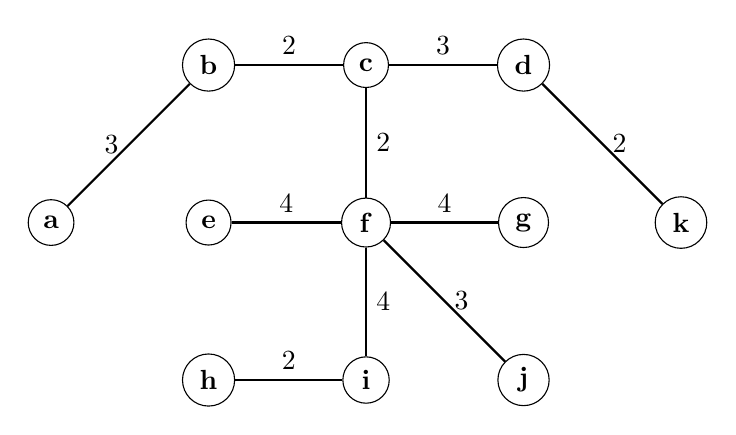
\begin{tikzpicture}
	
	\node[shape=circle,draw=black] (a) at (-2, 2)     {\textbf{a}};
	\node[shape=circle,draw=black] (b) at (0, 4)     {\textbf{b}};
	\node[shape=circle,draw=black] (c) at (2, 4)     {\textbf{c}};
	\node[shape=circle,draw=black] (d) at (4, 4)     {\textbf{d}};
	\node[shape=circle,draw=black] (e) at (0, 2)     {\textbf{e}};
	\node[shape=circle,draw=black] (f) at (2, 2)     {\textbf{f}};
	\node[shape=circle,draw=black] (g) at (4, 2)     {\textbf{g}};
	\node[shape=circle,draw=black] (h) at (0, 0)     {\textbf{h}};
	\node[shape=circle,draw=black] (i) at (2, 0)     {\textbf{i}};
	\node[shape=circle,draw=black] (j) at (4, 0)     {\textbf{j}};
	\node[shape=circle,draw=black] (k) at (6, 2)     {\textbf{k}};
	
	\path[-, thick] (a) edge node[left]{3} (b);
	\path[-, thick] (b) edge node[above]{2} (c);
	\path[-, thick] (c) edge node[above]{3} (d);
	\path[-, thick] (c) edge node[right]{2} (f);
	\path[-, thick] (d) edge node[right]{2} (k);
	\path[-, thick] (e) edge node[above]{4} (f);
	\path[-, thick] (f) edge node[above]{4} (g);
	\path[-, thick] (f) edge node[right]{4} (i);
	\path[-, thick] (f) edge node[right]{3} (j);
	\path[-, thick] (h) edge node[above]{2} (i);
	
	\end{tikzpicture} 
	\caption{Minimum Spanning Tree of Graph G.}	
	\label{fig:g4}
\end{figure}

\subsection*{c)} No it is not unique. Since there is another Minimum Spanning Tree with total weight 29.
\begin{figure}[H]
	\centering
	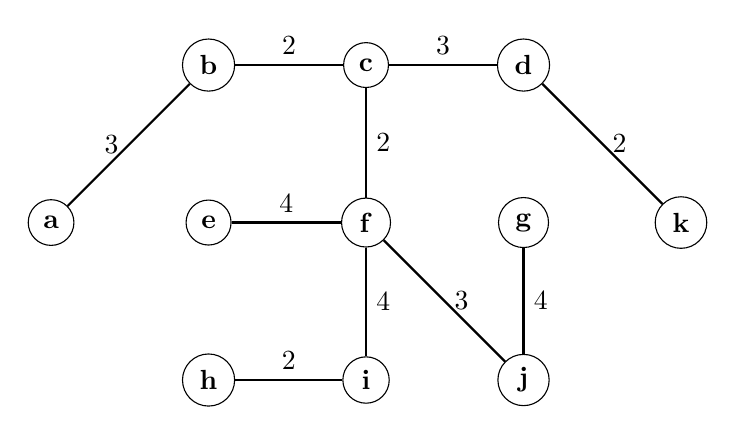
\begin{tikzpicture}
	
	\node[shape=circle,draw=black] (a) at (-2, 2)     {\textbf{a}};
	\node[shape=circle,draw=black] (b) at (0, 4)     {\textbf{b}};
	\node[shape=circle,draw=black] (c) at (2, 4)     {\textbf{c}};
	\node[shape=circle,draw=black] (d) at (4, 4)     {\textbf{d}};
	\node[shape=circle,draw=black] (e) at (0, 2)     {\textbf{e}};
	\node[shape=circle,draw=black] (f) at (2, 2)     {\textbf{f}};
	\node[shape=circle,draw=black] (g) at (4, 2)     {\textbf{g}};
	\node[shape=circle,draw=black] (h) at (0, 0)     {\textbf{h}};
	\node[shape=circle,draw=black] (i) at (2, 0)     {\textbf{i}};
	\node[shape=circle,draw=black] (j) at (4, 0)     {\textbf{j}};
	\node[shape=circle,draw=black] (k) at (6, 2)     {\textbf{k}};
	
	\path[-, thick] (a) edge node[left]{3} (b);
	\path[-, thick] (b) edge node[above]{2} (c);
	\path[-, thick] (c) edge node[above]{3} (d);
	\path[-, thick] (c) edge node[right]{2} (f);
	\path[-, thick] (d) edge node[right]{2} (k);
	\path[-, thick] (e) edge node[above]{4} (f);
	\path[-, thick] (j) edge node[right]{4} (g);
	\path[-, thick] (f) edge node[right]{4} (i);
	\path[-, thick] (f) edge node[right]{3} (j);
	\path[-, thick] (h) edge node[above]{2} (i);
	
	\end{tikzpicture} 
	\caption{Another Minimum Spanning Tree of Graph G.}	
	\label{fig:g4.1}
\end{figure}

\end{document}
